\section{Developer Experience, Sustainability, and Roadmap}
\label{sec:sustainability}

\subsection{Developer Experience and Infrastructure}
\label{sec:devex}

The development infrastructure is designed around one constraint: a project of
this scope spans many components with cross-cutting concerns, and the tooling
must make that manageable without forcing artificial coupling between parts
that should evolve independently.

\paragraph{Repository structure.}
The project uses a multi-repo layout under a single GitHub organization. Each
component has its own repository, its own release cycle, and its own CI
pipeline. Components can be updated independently as long as they do not
introduce breaking changes to the interfaces they expose. A breaking interface
change requires a coordinated update across all affected components, enforced
by the versioning mechanism described below.

\begin{lstlisting}[language=bash, caption={Repository structure}]
# Documentation and architecture
foundation              <- architecture document (this document)
wiki                    <- user-facing wiki, API reference landing page,
                           rustdoc/typedoc aggregation script

# OS image and distribution
distro                  <- mkosi configuration, ISO generation,
                           meta-packages, VM scripts, CI image pipeline,
                           top-level justfile, workspace-deps.toml
store-backend           <- Store API service, PostgreSQL schema,
                           object storage integration

# System layer
compositor              <- cosmic-comp fork (standalone repo, not a
                           GitHub fork; upstream tracked via git remote;
                           own patches maintained as numbered series in
                           patches/)
kernel-layer            <- eBPF programs only (aya, cross-compiled to
                           eBPF bytecode; developed and tested in VM only)
event-bus               <- Event Bus daemon, protobuf schema definitions,
                           Unix socket transport, event validation
knowledge               <- SQLite write store, Ladybug query store,
                           Graph Daemon, promotion pipeline
ai-layer                <- provider abstraction, MCP client, AI daemon
notification-daemon     <- Notification daemon (Rust)
install-daemon          <- Install Daemon, Integration Package matching

# Desktop and shell
desktop-shell           <- taskbar, Waypointer, Notification Center,
                           Quick Settings (Tauri + TypeScript)
app-lock-screen         <- Lock Screen (privileged context, own repo)
app-greeter             <- Greeter (runs before session, own repo)

# First-party applications
app-settings            <- Settings
app-files               <- File Manager
app-terminal            <- Terminal
app-store               <- Store
app-text-editor         <- Text Editor
app-system-monitor      <- System Monitor
app-wine-manager        <- Wine Manager
app-viewers             <- PDF Viewer, Image Viewer, Archive Manager

# Shared libraries
ui-kit                  <- component library, design token system
sdk                     <- os-sdk (Rust crate + TypeScript shell API for
                           first-party apps) and module-sdk (public subset,
                           re-exported from os-sdk; third-party modules);
                           single repo, two crates/packages, one version
themes                  <- GTK4 theme, Wine .msstyles, token source

# Community
community-integrations  <- community Integration Packages (PR-based,
                           CI validates schema)
community-adapters      <- community Settings Adapters (PR-based,
                           CI validates schema)
\end{lstlisting}

\paragraph{On GitHub.}
The project is hosted on GitHub. This requires an honest acknowledgment:
GitHub is owned by Microsoft, hosted in the United States, and therefore
structurally at odds with the project's European digital autonomy position.
The decision to use it is deliberate and time-limited, not an oversight.

Three factors make GitHub the right choice for the build phase. First,
network effects: the overwhelming majority of open-source contributors are
already on GitHub. Reducing the contribution barrier at the point when the
project most needs contributors is worth the sovereignty trade-off temporarily.
Second, tooling maturity: GitHub Actions, Dependabot, and the PR review
infrastructure are more reliable than the alternatives at this stage. Building
community around infrastructure problems is a distraction the project cannot
afford early on. Third, trust signal: a public GitHub repository with visible
activity, issues, and contributions is a credibility marker for a new project
asking users to run it as their operating system.

The migration path is planned and not open-ended.
\emph{Forgejo}~\cite{forgejo}, a fully open-source, self-hostable Git forge,
is the target for self-hosted source control. \emph{Codeberg}~\cite{codeberg},
a Forgejo-based hosting service operated by a German non-profit, is a viable
intermediate step. Git repositories are trivially portable; the harder
migration is Issues, PRs, and CI pipelines. That migration will be executed
when the project has the operational capacity to absorb it without disrupting
contributor workflows.

\paragraph{The \texttt{distro} repository.}
\texttt{distro} is responsible for everything that turns individual component
builds into a running operating system. It contains the mkosi configuration
declaring which packages and overlays go into the image, build scripts, VM
tooling for development and testing, meta-package RPM spec files, and the CI
pipeline that builds images on release candidates.

Two image build targets exist. The \emph{production image} contains no SSH
server, no debug symbols, and optimized binaries. This is what users receive.
The \emph{developer image} adds an SSH server, \texttt{debuginfo} packages,
Rust binaries compiled with debug symbols, and a known SSH key injected at
build time. It is only buildable via an explicit flag and is never distributed
as a release artifact.

\begin{lstlisting}[language=bash, caption={distro build targets}]
# Production image (default)
distro/build-image.sh

# Developer image with SSH and debug symbols
distro/build-image.sh --target developer

# Start a normal development VM
distro/run-vm.sh

# Mount a local directory into the VM via virtiofs
distro/run-vm.sh --share ~/projects/kernel-layer

# Start a persistent VM for update scenario testing
distro/vm-update-test.sh --init    # create persistent qcow2 disk
distro/vm-update-test.sh --start
distro/vm-update-test.sh --apply-update
distro/vm-update-test.sh --list-snapshots
distro/vm-update-test.sh --rollback
\end{lstlisting}

The update test target uses a \texttt{qcow2} disk image that persists across
VM restarts, enabling reproducible testing of the full Snapper snapshot,
health-check, and rollback cycle. The developer image is used as the base
for update tests so that SSH access and debug tooling are available during
the scenario.

A strict rule applies to eBPF development: eBPF programs are developed and
tested exclusively inside the VM, never directly on the development machine.
A bad eBPF program can destabilize the kernel; the VM isolation is not
optional.

\paragraph{Build system.}
\emph{mkosi}~\cite{mkosi}, maintained by the systemd team, is the target
tool for image generation. It builds bootable OS images from a declarative
configuration file that specifies which packages to include, which overlay
files to add, and how to configure the system. Unlike Kickstart or Kiwi, mkosi
is designed around the systemd ecosystem: it integrates directly with
\texttt{systemd-repart} for partition layout and produces well-formed UEFI
images that support Secure Boot and Unified Kernel Images without custom glue
scripts. It supports multiple output formats: ISO, raw disk image, and
container. It integrates cleanly with the Open Build Service. Confirming that
mkosi handles the full build pipeline in practice is an open item pending
actual use.

\emph{just}~\cite{just} is the task runner for all development and CI
workflows. Unlike \texttt{make}, \texttt{just} has no implicit rules, no
file-dependency semantics, and no whitespace pitfalls. Every task is an
explicit named recipe. The \texttt{distro} repository contains the top-level
\texttt{justfile} that serves as the single entry point for all common
operations:

\begin{lstlisting}[language=bash, caption={Top-level just recipes (distro repo)}]
just dev          # start Event Bus, Graph Daemon, and shell daemons
                  # in the current session for daemon-level development
just test         # run unit tests across all repos in dependency order
just build-iso    # produce a production ISO via mkosi
just build-dev    # produce a developer ISO with SSH and debug symbols
just vm           # boot the developer ISO in QEMU with KVM acceleration
just vm-nested    # run the shell inside the current Wayland session
                  # (no VM; compositor-level development only)
just vm-debug     # boot with GDB server exposed on port 1234
just bench        # run graph-scale benchmarks against synthetic datasets
just check-deps   # verify all repos are on the pinned dependency versions
\end{lstlisting}

Component repositories each have their own \texttt{justfile} for
component-specific tasks. The top-level \texttt{justfile} delegates to them
and handles cross-repo orchestration. A developer working on a single
component never needs to leave that repository; the top-level recipes exist
for integration work and release builds.

The Rust codebase is organized into three Cargo workspaces, each scoped to
a deployment boundary rather than an architectural layer. The
\emph{system workspace} contains components that run with elevated privileges
or as system daemons: \texttt{event-bus}, \texttt{kernel-layer},
\texttt{knowledge}, \texttt{ai-layer}, \texttt{notification-daemon}, and
\texttt{install-daemon}. The \emph{desktop workspace} contains components
that run in the user session: \texttt{compositor}, \texttt{desktop-shell},
\texttt{sdk}, and \texttt{app-lock-screen}. The \emph{apps workspace} contains
first-party applications. Cross-workspace dependencies are only permitted
over stable IPC interfaces, never via Cargo path dependencies. This boundary
is enforced by the workspace structure: a component in the system workspace
cannot import a crate from the desktop workspace at compile time.

The \emph{Open Build Service}~\cite{obs} (OBS) handles packaging for all
custom components. OBS is an openSUSE-hosted build infrastructure that takes
RPM spec files and produces binary packages for multiple distributions and
architectures in parallel, without requiring the developer to provision
build machines for each target. Packages are signed with the project GPG
key; \emph{GPG} (GNU Privacy Guard~\cite{gnupg}) is the standard
open-source implementation of the OpenPGP signing and encryption standard;
package signatures let end-user systems verify that a package was built and
signed by this project and has not been tampered with. OBS hosts the resulting
package repository that end-user systems pull from. Both Fedora and OpenSUSE
targets can be built from the same spec files, which is one practical reason
both remain viable candidates.

\paragraph{Update system.}
Updates arrive from two independent streams managed separately. The base
system, meaning the kernel and base distribution packages, is handled by the
native package manager (dnf), with
Snapper automatically taking a Btrfs snapshot before every update. Project
components, meaning the compositor, shell, event bus, graph daemon, AI layer,
and first-party applications, are distributed via the project's own OBS
repository as RPM packages managed as a coordinated meta-package.

The update behavior is designed to be non-intrusive. Security updates for both
streams are downloaded automatically in the background and applied at the next
shutdown or reboot, never during an active session. No forced reboots, no
countdown timers. All other updates are downloaded silently in the background;
a single calm notification appears when they are ready. The user applies them
when convenient. In managed environments, administrators can configure mandatory
update windows; even then, no mid-session interruption occurs.

Rollback is available for every update: Btrfs and Snapper record a snapshot
before each change, and the user can boot into a previous snapshot from the
boot menu and roll back the entire system without any additional tooling.

Project components communicate over defined IPC interfaces. A breaking
interface change increments the major version number and must be shipped as a
coordinated meta-package update, so that incompatible component versions cannot
coexist. Components verify interface compatibility at startup:

\begin{lstlisting}[language=Rust, caption={Interface compatibility check at startup}]
fn check_compatibility() -> Result<()> {
    let daemon_version = get_graph_daemon_version()?;
    if daemon_version.major != EXPECTED_MAJOR {
        bail!("Graph Daemon interface version mismatch. Run system update.");
    }
    Ok(())
}
\end{lstlisting}

A component that detects a version mismatch refuses to start and surfaces a
clear message. The only resolution is applying the pending system update.

\paragraph{Hosting infrastructure.}
The project operates two distinct distribution channels with different
infrastructure requirements.

\emph{System package repository.} All core system components, comprising the compositor,
shell, daemons, and first-party applications, are distributed as RPMs via the
Open Build Service. OBS builds, signs, and hosts the repository. End-user
systems add the repository once:

\begin{lstlisting}[language=bash]
dnf config-manager --add-repo \
    https://packages.[project].dev/fedora/$releasever/
\end{lstlisting}

After that, updates arrive through the normal \texttt{dnf} update mechanism.
No custom infrastructure is required for this channel; OBS provides everything.

\emph{Store backend.} The Store requires purpose-built infrastructure because
its requirements are specific to this project: Integration Package matching,
adapter schema validation, the rating-based Install Daemon policy, signed
package verification, and payment processing. The target stack is a Rust
backend service with PostgreSQL for metadata and S3-compatible object storage
for package binaries. \emph{Hetzner Object Storage} is the preferred object
storage provider: it is operated in European data centres, priced predictably
for outbound traffic, and S3-compatible without vendor lock-in. A CDN sits in
front of the object storage for binary downloads; \emph{BunnyNet} is the
preferred provider for the same reasons.

Payment processing uses \emph{Stripe}, which covers European payment standards,
handles VAT for digital goods across EU jurisdictions, and provides a
well-documented API. Stripe's commission is accounted for separately from the
Store's own commission tiers described in Section~\ref{sec:store}.

The Store backend is self-hosted, not dependent on any US-based platform
service for its critical path. This is a direct consequence of the project's
European digital autonomy stance: the infrastructure that distributes software
to users should be under the project's control and subject to European law.

\paragraph{CI/CD pipeline.}
Every repository inherits a shared CI template maintained in
\texttt{foundation}. The template defines the required jobs; repositories can
add jobs but cannot remove or weaken the required set. This ensures a uniform
quality gate across all components without duplicating workflow configuration.

Tests run at four levels of integration.

\emph{Unit tests} run on every push and every pull request, per repository,
with a target runtime under 60 seconds. All external dependencies are mocked
using the official mocks from \texttt{sdk}. Rust components use
\texttt{cargo test}; TypeScript components use \emph{Vitest}~\cite{vitest},
a Vite-native test framework with Jest-compatible API. No pull request merges
without green unit tests.

\emph{Integration tests} run on every merge to \texttt{main}, per repository,
with a target runtime under 5 minutes. They start the directly involved
daemons as real subprocesses against real Unix sockets and verify end-to-end
behavior without a full system boot. A failing integration test with passing
unit tests indicates interface drift between repositories, which is the primary
failure mode this level exists to catch. Representative examples: an event
emitted by the Event Bus lands correctly as a node in Ladybug after the
promotion pass; a theme token change propagates from Settings to all running
Tauri processes; a keybinding action dispatched by the shell reaches the
correct handler in the Input Manager.

\emph{eBPF tests} are a special case. eBPF programs require a real kernel with
\texttt{CAP\_BPF} and BTF support; they cannot run against mocks. Rather than
requiring a dedicated self-hosted runner, the CI job uses nested virtualization
available on standard GitHub Actions Ubuntu runners: a minimal QEMU instance
is started inside the CI job, eBPF tests run inside it, and the VM is
discarded on completion. This adds approximately 15 seconds of overhead per
run. eBPF tests run on every merge to \texttt{main} in the
\texttt{kernel-layer} repository only.

\emph{System tests} boot a complete ISO in QEMU and run a defined smoke
scenario: system boots without crash; Waypointer opens and launches an
application; eBPF events arrive in the Knowledge Graph; theme switch
propagates; module install and uninstall complete correctly. These tests are
slow (15 to 30 minutes) and run only on release candidates, triggered
manually. The ISO is built by the same mkosi configuration used for real
releases; there is no separate test image. A caching mechanism in
\texttt{distro} stores the base image between runs and invalidates it only
when \texttt{distro} or \texttt{kernel-layer} changes; component-only updates
patch the cached image rather than rebuilding from scratch.

\emph{Interface compatibility checks} run on every pull request that touches
a public API. For Rust-to-Rust interfaces, a stored baseline of the generated
protobuf bindings and \texttt{sdk} types is compared against the proposed
change; a breaking change without a major version bump causes the check to
fail. For the Rust-to-TypeScript boundary in \texttt{sdk}, the
\texttt{ts-rs}~\cite{ts-rs} crate generates TypeScript type definitions
directly from Rust structs via derive macros. The generated \texttt{.ts} files
are committed to the repository. CI verifies that the committed files match
the output of a fresh \texttt{cargo build}; a mismatch means the Rust types
were changed without regenerating the bindings. This eliminates an entire
class of runtime type mismatches between the Rust backend and the TypeScript
frontend.

\emph{Graph performance benchmarks} run after every merge to \texttt{main}
in the \texttt{knowledge} repository. Using \texttt{criterion}~\cite{criterion},
the benchmark suite exercises the most common query patterns against synthetic
graphs of three sizes: 1,000 nodes, 50,000 nodes, and 500,000 nodes. The
benchmark results are stored as GitHub Actions artifacts, providing a
longitudinal record of query latency as the codebase evolves. The benchmark
does not automatically fail the build; it produces a comment on the merge
commit with the delta against the previous run. Automatic failure is triggered
only if latency exceeds twice the established baseline, indicating a
significant regression rather than normal variance.

Table~\ref{tab:ci-triggers} summarizes when each level runs.

\begin{table}[htbp]
\caption{CI trigger summary}
\label{tab:ci-triggers}
\begin{tabularx}{\linewidth}{lX}
\toprule
\textbf{Trigger} & \textbf{What runs} \\
\midrule
Every push or pull request     & Unit tests; interface compatibility check if public API touched \\
Merge to \texttt{main}         & Unit tests, lint, clippy, integration tests \\
Merge to \texttt{main} in \texttt{kernel-layer} & Above plus eBPF tests in QEMU \\
Merge to \texttt{main} in \texttt{knowledge}    & Above plus graph performance benchmark \\
Release candidate (manual)     & Full system tests in QEMU \\
Weekly (scheduled)             & Upstream cosmic-comp rebase check; dependency drift check \\
\bottomrule
\end{tabularx}
\end{table}

\paragraph{Local development workflow.}
Development happens at three levels of integration, each suited to a different
class of work. The common case is developing a single component in isolation.
Each repository has its own development setup with \texttt{cargo run},
\texttt{tauri dev}, or hot-reload as appropriate. Components that use the mocks
from \texttt{os-sdk} need no external dependencies running. Fast feedback loop,
runs entirely on the developer's machine.

For shell and compositor work, the cosmic-comp fork supports nested mode: the
compositor runs as a regular Wayland window inside the developer's existing
desktop. The full shell appears inside that window. No VM or extra hardware is
needed. This covers the majority of shell and compositor development; eBPF and
kernel-level components are not active in nested mode.

Full system work requires \emph{QEMU}~\cite{qemu}, a machine emulator and
virtualizer. QEMU can emulate a complete x86-64 machine, including CPU, RAM, storage,
network, and display, entirely in software, or accelerate execution via KVM
(the Linux kernel's hardware virtualization support) to near-native speed when
running on matching hardware. This covers eBPF development, the boot sequence,
the update system, and anything that requires a real kernel or a complete
system environment. The \texttt{distro} repository contains the full script
set for this workflow, described in the \texttt{distro} paragraph above.

\paragraph{Mock strategy.}
Every IPC interface in the system has an official mock implementation that
lives in \texttt{os-sdk} directly alongside the interface definition. Mock and
real implementation share the same type definitions. An outdated mock is a
build error, not a runtime surprise: if an interface changes, the mock must be
updated in the same pull request.

\begin{lstlisting}[language=Rust, caption={Conditional mock usage in tests}]
#[cfg(test)]
use os_sdk::graph_daemon::mock::GraphDaemonMock as GraphDaemon;

#[cfg(not(test))]
use os_sdk::graph_daemon::client::GraphDaemonClient as GraphDaemon;
\end{lstlisting}

There are no per-repository custom stubs and no fixture files that can drift
from the real schema. The mock is the contract.

\paragraph{Dependency management.}
Shared dependencies across repositories are pinned in a
\texttt{workspace-deps.toml} file in the \texttt{distro} repository. This
file declares the authoritative versions of common crates (tokio, serde,
protobuf, and others) that all repositories are expected to use. A
\texttt{check-deps} recipe in the top-level \texttt{justfile} verifies that
every repository's \texttt{Cargo.toml} matches the pinned versions and fails
with a diff if not. Dependabot runs only on the \texttt{distro} repository
and opens pull requests against \texttt{workspace-deps.toml}. When such a
pull request merges, a workflow automatically opens follow-up pull requests in
all affected repositories updating them to the new version. No repository
manually tracks shared dependency versions; all version decisions flow
downstream from \texttt{distro}.

\paragraph{Compositor upstream tracking.}
The \texttt{compositor} repository tracks the cosmic-comp upstream as a git
remote named \texttt{upstream}. The project's own modifications are maintained
as a numbered patch series in \texttt{compositor/patches/}, following the
convention established by projects such as OpenWRT and Buildroot:

\begin{lstlisting}[language=bash, caption={Compositor patch series structure}]
compositor/patches/
  0001-remove-cosmic-shell-ipc.patch
  0002-add-custom-event-socket.patch
  0003-expose-focus-events-to-event-bus.patch
\end{lstlisting}

A weekly scheduled CI job attempts to rebase the patch series onto the latest
\texttt{upstream/main}. If the rebase fails, the job opens a GitHub issue
identifying the specific patch that produced the conflict. If it succeeds, the
rebased branch is proposed as a pull request for review before merging. This
surfaces upstream conflicts immediately rather than accumulating them silently.

Any modification that does not require project-specific behavior is submitted
as a pull request to the cosmic-comp upstream repository first. If accepted,
it is removed from the patch series. Keeping the patch series as short as
possible is an explicit maintenance goal; every patch that gets accepted
upstream is one less patch to rebase.

\paragraph{Secrets management.}
A \texttt{secrets.env.example} file in the \texttt{distro} repository
documents every environment variable that CI and release tooling require, with
a description and a placeholder value. CI jobs reference only environment
variables, never hardcoded secret names from any specific secret store. A
single mapping file translates the CI platform's secret storage (currently
GitHub Actions Secrets) to the canonical variable names. Migrating to a
different CI platform or secret store requires changing only this mapping file;
no workflow or script elsewhere in the codebase references platform-specific
secret syntax.

\paragraph{Project planning tooling.}
A project of this scope has cross-cutting concerns that span multiple
repositories simultaneously: an Epic about the Waypointer Module API touches
\texttt{desktop-shell}, \texttt{os-sdk}, \texttt{module-sdk}, and potentially
\texttt{compositor}. Standard per-repository issue tracking is not sufficient
for this. The requirements are hierarchical issues or Epics that span multiple
repositories, dependency tracking between issues, a roadmap view across all
components, and cross-repository milestone coordination.

Three options are under evaluation. The first is GitHub Projects v2 with a
meta-repo convention: cross-cutting Epics live as issues in the
\texttt{foundation} repository and component repositories link back to the
relevant Epic; GitHub Projects v2 aggregates issues from all repositories into
one board. The advantage is zero additional tooling and everything staying
in GitHub. The disadvantage is that dependency tracking is honor-system only
with no enforcement, there is no proper roadmap view, and Epic-to-child
linking is manual.

The second option is \emph{Linear}~\cite{linear}, a proprietary hosted tool
with strong multi-repo GitHub integration, real Epics with child issues, a
dependency graph, and a roadmap view. It has the best user experience for
exactly this use case but is proprietary, hosted externally, and costs money
at team scale.

The third is \emph{Plane}~\cite{plane}, an open-source Linear alternative
that can be self-hosted. Feature parity with Linear is growing but not yet
complete. Its advantage is that self-hosting fits the project's digital
sovereignty philosophy with no external dependency; the disadvantage is
additional operational overhead and some features that are still maturing.

The decision is not yet made. The requirement is clear: cross-repository Epic
tracking with dependency enforcement and a roadmap view. GitHub Projects alone
is likely insufficient for a project of this scope.

\paragraph{Documentation.}
Two documentation sites are maintained, both self-hosted. The user-facing wiki
at \texttt{wiki.[project].dev} is written by hand in the spirit of the Arch
Wiki: prose that explains intent and reasoning, not only what a setting does.
It covers concepts, how-tos, troubleshooting, and architecture explanations.
Community contributions are accepted via pull requests reviewed by the core
team. The wiki source lives in the \texttt{wiki} repository, separate from
\texttt{foundation} which contains only the architecture document.

The developer API reference at \texttt{api.[project].dev} is auto-generated
from code comments: \texttt{rustdoc} for Rust components,
\texttt{typedoc} for TypeScript components, aggregated and hosted under a single
domain so there is one place to search across all components. The aggregation
script and the API reference landing page live in \texttt{wiki} alongside the
user-facing documentation; both sites share the same visual language and are
maintained together. Keeping the API reference current is a CI gate: a pull
request that removes or modifies a public API without updating its documentation
comment does not merge.

\subsection{Sustainability and Business Model}
\label{sec:business}

This is an open source project. The code is and remains open; that is a
foundational commitment, not a marketing position. At the same time, building
and maintaining a full operating system is a serious engineering effort that
requires sustained funding. The goal is not to extract value from users but to
find revenue streams that are structurally aligned with the project's values:
user sovereignty, transparency, and European digital autonomy.

\paragraph{Principles.}
Four constraints rule out entire categories of business models upfront. Core
OS functionality is not feature-gated behind a paywall; the desktop, the
permission system, the Knowledge Graph, and the AI layer are open and available
to everyone. There is no advertising, no telemetry sold to third parties, and
no data brokering. Venture capital with growth-at-all-costs expectations is
incompatible with a project built on user trust and is therefore excluded.
Enterprise features are an acceptable source of revenue; making the core worse
for non-paying users is not.

\paragraph{Store revenue.}
The Store's tiered commission model, described in Section~\ref{sec:store},
generates revenue proportional to ecosystem health. The project earns
meaningfully only if developers earn well first. At early stage this is
negligible. At meaningful adoption it becomes a significant funding stream. The
Store handles application sales, theme sales, module distribution, and profile
package distribution under a single infrastructure.

\paragraph{Enterprise services.}
The Signed Profile Package system described in Section~\ref{sec:profiles} is
already designed with organizations in mind. The \texttt{.lenv} format is open
and documented; anyone can author packages. Organizations deploying managed
environments at scale will often want professional help: authoring and
maintaining custom packages, deployment tooling, update management, and support
SLAs. This is a natural B2B offering that does not touch the open source core.
The analogy is Red Hat selling support for software that anyone can download
for free.

\paragraph{OEM and hardware partnerships.}
At sufficient maturity and hardware compatibility, small European laptop
manufacturers may want to ship the system pre-installed. The structural
alignment is good: the manufacturer gets a differentiated product, users get a
well-tested hardware and software combination, and the project gets sustainable
revenue from certification and validation work and an ongoing support
relationship. This requires a stable release and a polished out-of-box
experience first and is a longer-term play. Relevant candidates in the European market include
\emph{Tuxedo Computers}~\cite{tuxedo}, the \emph{PINE64}~\cite{pine64}
ecosystem, and potential \emph{Framework}~\cite{framework} partnerships.

\paragraph{Support tiers.}
A support subscription aimed at power users, small businesses, and developers
who want guaranteed response times and direct access offers prioritized bug
reports, LTS release guarantees with defined support windows, and a direct
communication channel with the core team. No features are locked behind this;
it is a service layer on top of the open product, priced modestly enough to be
accessible to individual developers.

\paragraph{Public funding and grants.}
The European open source and digital sovereignty funding landscape is
underutilized by most projects. The \emph{Sovereign Tech Fund}~\cite{stf} in Germany funds open source
infrastructure projects and explicitly values work that reduces dependency on
US technology monopolies. The \emph{NLnet Foundation}~\cite{nlnet} funds internet and open source
projects with a privacy and user rights focus and has supported numerous small
to medium projects. The \emph{NGI} (Next Generation Internet~\cite{ngi}) programme runs
multiple EU funding calls per year for open source, privacy, and
decentralization work.

The European digital autonomy angle is not only a philosophical position; it is
a genuine funding argument. A European open source operating system built on
sovereignty principles is precisely what these programmes exist to support.
Grants do not provide recurring revenue but they can fund specific development
phases without creating investor obligations or governance compromises.

\paragraph{Path to incorporation.}
A company makes sense when there is external money to manage, not before.
Premature incorporation adds administrative overhead with no corresponding
benefit. A realistic sequence: the project gains traction and a community
forms; grant applications are filed; Store revenue starts, providing the first
external money flow; the first enterprise inquiry for deployment support
arrives as the first B2B signal. At that point incorporation becomes
appropriate, probably as a GmbH in Austria or Germany, or as a European
cooperative structure if community governance is a priority.

The company's role is to employ core contributors, manage the Store
infrastructure, and sell enterprise and support services. The open source
project remains governed independently of the company: contribution policy,
release decisions, and core architecture are not dictated by commercial
interests. This separation must be written down explicitly before the company
is incorporated, not negotiated afterward under time pressure.

\subsection{Roadmap}
\label{sec:roadmap}

The system has two independent development tracks that converge at a defined
integration point. The \emph{data track} covers kernel instrumentation, the
event pipeline, and the Knowledge Graph: components that can be built, tested,
and benchmarked without any desktop present. The \emph{desktop track} covers
the compositor fork and the shell: components that require a Wayland environment
but not a working graph. The tracks run in parallel through Phase~2; they
merge in Phase~3 when the graph is connected to the shell for the first time.

\begin{figure}[htbp]
\centering
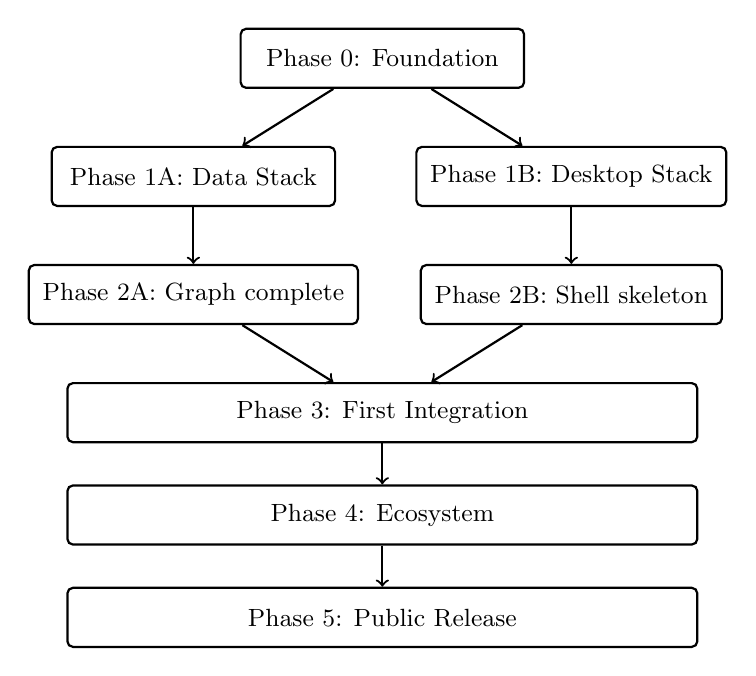
\begin{tikzpicture}[
  box/.style={
    draw, thick, rectangle, rounded corners=2pt,
    minimum width=3.6cm, minimum height=0.75cm,
    font=\small, align=center, inner sep=5pt
  },
  merge/.style={
    draw, thick, rectangle, rounded corners=2pt,
    minimum width=8.0cm, minimum height=0.75cm,
    font=\small, align=center, inner sep=5pt
  },
  arr/.style={->, thick},
  lbl/.style={font=\footnotesize\itshape},
]

\node[box] (p0)    at (0, 5.0)  {Phase 0: Foundation};

\node[box] (p1a)   at (-2.4, 3.5) {Phase 1A: Data Stack};
\node[box] (p1b)   at ( 2.4, 3.5) {Phase 1B: Desktop Stack};

\node[box] (p2a)   at (-2.4, 2.0) {Phase 2A: Graph complete};
\node[box] (p2b)   at ( 2.4, 2.0) {Phase 2B: Shell skeleton};

\node[merge] (p3)  at (0, 0.5)  {Phase 3: First Integration};
\node[merge] (p4)  at (0, -0.8) {Phase 4: Ecosystem};
\node[merge] (p5)  at (0, -2.1) {Phase 5: Public Release};

\draw[arr] (p0)  -- (p1a);
\draw[arr] (p0)  -- (p1b);
\draw[arr] (p1a) -- (p2a);
\draw[arr] (p1b) -- (p2b);
\draw[arr] (p2a) -- (p3);
\draw[arr] (p2b) -- (p3);
\draw[arr] (p3)  -- (p4);
\draw[arr] (p4)  -- (p5);

\end{tikzpicture}
\caption{Phase dependency structure. Phases~1 and~2 run as parallel tracks;
neither blocks the other. Phase~3 is the first point at which both tracks must
be simultaneously stable. Phases~4 and~5 are sequential.}
\label{fig:roadmap}
\end{figure}

Three types of milestone appear in each phase. \emph{Technical gates} are
binary, automatically verifiable conditions that must pass before the next
phase begins: a specific CI job is green, a benchmark hits a defined threshold,
or an interface check passes. \emph{UX milestones} are qualitative judgments
about usability that require a human to verify: a defined task completed
without assistance by a target user type. \emph{Sustainability milestones}
track organizational and community progress that runs in parallel with
technical development.

\paragraph{Phase 0: Foundation (current).}
Architecture and design decisions are documented in this blueprint. The
repository organization, CI template, and shared tooling are established before
component code is written. The base distribution is Fedora. The
\texttt{event-bus} protobuf schema is defined; the \texttt{sdk} crate structure
is initialized with the public API as traits before any implementation exists.
This ordering is intentional: schema and interface decisions are the most
expensive to change once downstream components exist.

\emph{Technical gates:} SQLite write store sustains 5,000 synthetic events per
second under continuous load without data loss; promotion pipeline moves events
into Ladybug and a Cypher query returns correct results; CI template deployed
and all initial repositories pass the required jobs; \texttt{just dev} starts
the Event Bus and Graph Daemon locally in under 10 seconds.

\emph{Sustainability milestones:} GitHub organization created with all
repositories; \texttt{foundation} repository public with this document;
ORCID and Zenodo record created for the architecture document.

\paragraph{Phase 1A: Data Stack.}
The eBPF Normalizer is operational, deduplicating and filtering raw kernel
events before they reach the Event Bus. The promotion pipeline is stable under
real desktop load, not only synthetic load. The Graph Daemon exposes a complete
Cypher query interface over its Unix socket. All components have integration
tests that run against real IPC sockets. The \texttt{knowledge} benchmark
suite is established and producing baseline measurements.

eBPF programs are developed and tested exclusively inside the QEMU developer
VM from this point forward. A bad eBPF program can produce a kernel panic; VM
isolation is mandatory, not optional.

\emph{Technical gates:} eBPF test job green in CI using nested QEMU on GitHub
Actions runners; integration test suite passes for the full pipeline from raw
eBPF event to Ladybug node; graph query latency baseline established for 1k,
50k, and 500k node datasets.

\paragraph{Phase 1B: Desktop Stack.}
The \texttt{compositor} repository is initialized as a standalone fork of
cosmic-comp with the COSMIC shell IPC removed and the custom Event Bus socket
added as the first patch in the series. The upstream tracking process is
operational: the weekly rebase CI job runs, and the patch series is clean
against current upstream. The compositor runs in nested mode inside an existing
Wayland session. No shell is connected yet.

\emph{Technical gates:} compositor starts in nested mode without crash;
upstream rebase CI job runs and produces no conflicts against current
\texttt{upstream/main}; patch series contains no more than five patches.

\paragraph{Phase 2A: Graph Complete.}
The full Knowledge Graph schema is implemented and stable. All node types
documented in Section~\ref{sec:knowledge-graph} exist and are populated by
real system activity. The temporal filesystem view at
\texttt{\textasciitilde/.timeline/} is functional. Retention policy and
summarization are implemented. The Graph Daemon is considered feature-complete
for the purposes of AI layer integration.

\emph{Technical gates:} all node types populated from a 24-hour real usage
session; \texttt{\textasciitilde/.timeline/} lists correct files for a
given date; retention pass runs and compacts nodes correctly.

\paragraph{Phase 2B: Shell Skeleton.}
The shell runs on the compositor fork. The taskbar, Waypointer (without graph
integration), the global menu bar, and the Appearance section of Settings are
functional. The theme system is operational: token-based switching propagates
to all Tauri surfaces and GTK4 applications. A developer can use this
environment as a basic desktop without requiring a terminal for routine tasks.

\emph{Technical gates:} Panda, Light, Dark, and High Contrast themes all
apply correctly and switch without a session restart; Waypointer launches
applications; the global menu bar renders menus from a first-party application.

\emph{UX milestone:} a developer who did not build the system can complete
five predefined tasks using only the shell, without referring to documentation.

\paragraph{Phase 3: First Integration.}
The two tracks are connected. Waypointer queries the Knowledge Graph for recent
files and project context. Focus Mode is fully implemented. The AI Daemon
operates with a local provider. The Connections system and Settings AI category
are functional. This is the first phase where the system is used as a daily
driver by the primary developer.

The daily driver criterion is not aspirational language. It is a concrete
testing strategy: running the system as the primary work environment for a
minimum of 30 consecutive days surfaces bugs and rough edges that no scripted
test scenario will find.

\emph{Technical gates:} Waypointer returns graph-sourced recent files
correctly; Focus Mode activates and deactivates all documented side effects;
AI Daemon responds to a graph query with a local provider configured.

\emph{UX milestone:} a non-technical test user completes a defined set of
daily tasks (web browsing, document editing, file management, calendar review)
without opening a terminal and without asking for help.

\emph{Sustainability milestones:} first public blog post or video documenting
the project; Sovereign Tech Fund and NLnet grant applications submitted.

\paragraph{Phase 4: Ecosystem.}
The Store is operational. The Install Daemon handles Integration Package
matching. The Module Runtime is functional. The first external developers are
onboarded with documentation and the \texttt{module-sdk}. Signed Profile
Packages for managed environments are supported. The project planning tool
decision is made and the chosen tool is in use.

\emph{Technical gates:} a Store application submitted by a developer outside
the core team installs and runs correctly end-to-end; a module declared in a
\texttt{.project} file activates and deactivates with Focus Mode.

\emph{UX milestone:} an external developer builds and submits a Store
application using only the published documentation, without asking the core
team for help.

\emph{Sustainability milestones:} first external contributor with a merged
pull request; Store infrastructure operational on Hetzner; first grant
funding received or first enterprise inquiry received.

\paragraph{Phase 5: Public Release.}
No new features. Hardware compatibility is validated against a defined target
list. The Nvidia first-boot detection and driver installation flow is tested on
real hardware. The installer is polished and the out-of-box experience meets
the bar set in Phase~3's UX milestone at scale. Documentation covers
installation, first use, and the most common troubleshooting scenarios.

\emph{Technical gates:} system tests green on release candidate ISO; Nvidia
driver flow completes without manual intervention on a tested device; installer
completes without errors on three distinct hardware configurations.

\emph{UX milestone:} a non-technical user installs the system from USB without
reading any documentation beyond the installer prompts, and reaches a working
desktop.

\emph{Sustainability milestones:} migration timeline from GitHub to
Forgejo/Codeberg defined; incorporation decision made based on available
funding and community size.
